% use `pdflatex -shell-escape Perfect_Circumplex.tex` in the terminal

\documentclass[crop,tikz,convert={outext=.svg,command=\unexpanded{pdf2svg \infile\space\outfile}},multi=false]{standalone}
\usepackage{xcolor}
\usepackage{tikz}
\usetikzlibrary{calc,arrows,positioning}
\usetikzlibrary{shapes.geometric,arrows,positioning}
\definecolor{phg}{HTML}{8CD000} % Coporate Design Green


\renewcommand{\familydefault}{\sfdefault}
\usepackage[]{mathastext} %% Hat noch die option [italic]
% 'isomath' sets upper case greek letters italic in accordance with 
% the International Standard ISO 80000-2
%\usepackage{isomath}


\begin{document}
\tikzset{ % set color globally
  every picture/.append style={
    color=phg,
  }
}

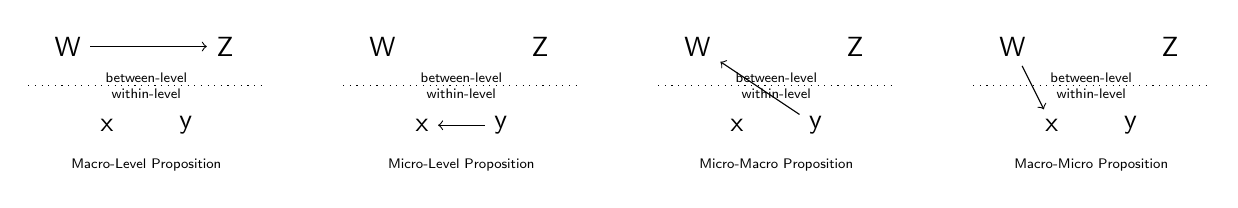
\begin{tikzpicture}

\node (W) at (-1,.5) {W};
\node (Z) at ( 1,.5) {Z};

\node (t) at ( 0,.1) {\tiny between-level};
\draw[dotted] (-1.5,0) -- (1.5,0);
\node (t) at ( 0,-.1) {\tiny within-level};

\node (x) at (-.5,-.5) {x};
\node (y) at ( .5,-.5) {y};

\draw[->] (W) -- node {} (Z);

\node (t) at ( 0,-1) {\tiny Macro-Level Proposition};

%%%%%%%%%%%%%%%
\begin{scope}[shift={(4, 0)}]
\node (W) at (-1,.5) {W};
\node (Z) at ( 1,.5) {Z};

\node (t) at ( 0,.1) {\tiny between-level};
\draw[dotted] (-1.5,0) -- (1.5,0);
\node (t) at ( 0,-.1) {\tiny within-level};

\node (x) at (-.5,-.5) {x};
\node (y) at ( .5,-.5) {y};

\draw[->] (y) -- node {} (x);

\node (t) at ( 0,-1) {\tiny Micro-Level Proposition};
\end{scope}

%%%%%%%%%%%%%%%
\begin{scope}[shift={(8, 0)}]
\node (W) at (-1,.5) {W};
\node (Z) at ( 1,.5) {Z};

\node (t) at ( 0,.1) {\tiny between-level};
\draw[dotted] (-1.5,0) -- (1.5,0);
\node (t) at ( 0,-.1) {\tiny within-level};

\node (x) at (-.5,-.5) {x};
\node (y) at ( .5,-.5) {y};

\draw[->] (y) -- node {} (W);

\node (t) at ( 0,-1) {\tiny Micro-Macro Proposition};
\end{scope}

%%%%%%%%%%%%%%%
\begin{scope}[shift={(12, 0)}]
\node (W) at (-1,.5) {W};
\node (Z) at ( 1,.5) {Z};

\node (t) at ( 0,.1) {\tiny between-level};
\draw[dotted] (-1.5,0) -- (1.5,0);
\node (t) at ( 0,-.1) {\tiny within-level};

\node (x) at (-.5,-.5) {x};
\node (y) at ( .5,-.5) {y};

\draw[->] (W) -- node {} (x);

\node (t) at ( 0,-1) {\tiny Macro-Micro Proposition};
\end{scope}

      
\end{tikzpicture}

\end{document} 